\documentclass[12pt]{report}
\usepackage[utf8]{inputenc}
\usepackage[T1]{fontenc} %font encoding for some characters
\usepackage{csquotes}
\usepackage[french]{babel} %give french translation for most commands
\usepackage{fullpage} %extend document's text width
\usepackage[
style=numeric,
backend=biber,
sortlocale=fr-FR,
language=french,
sorting=none %permet de classer la bibliographie dans l'ordre de citation
]{biblatex}
\addbibresource{bibliographie.bib}
\usepackage{graphicx} %make usage of images simpler
\usepackage{lastpage} %make a usable reference to the lastpage
\usepackage{subfigure} %enable to produce subfigure in figure environment
\usepackage{multicol} %enable multi-columns part easily
\usepackage{lmodern} %some more characters encoding stuff
\usepackage{enumitem} %enable label modification for lists
\usepackage[bottom, perpage]{footmisc} %reset footnote counter each page
\usepackage{tabulary} %able to use tabulary env or set column width in tabular
\usepackage[hidelinks]{hyperref} %enable links creation into the pdf
\usepackage[toc, acronym]{glossaries} %generate glossary with entries used with \gls. Needs to be loaded after hyperref for clickable links
\usepackage[
    disable,% uncomment this when finished
    french,
    colorinlistoftodos,
    backgroundcolor=blue!40
]{todonotes} %todo list to complete the document
\usepackage{fancyhdr}
\usepackage{float}
\usepackage{lipsum} %generate lorem ipsum
\usepackage{refcount} %used to get refpage as number
\usepackage{xintexpr} %used to have boolean expression
\usepackage{url}
%\usepackage[ddmmyyyy]{datetime} %used for custom \today cmd
\setrefcountdefault{-1} %used to set pagref during compile time


\let\cleardoublepage\clearpage

\setlength{\headsep}{2pt}
\nocite{*} %permet d'écrire toutes les entrées présentes dans la bibliographie sans avoir à les citer
\glsaddall %permet d'écrire toutes les entrées présentes dans le glossaire sans avoir à les citer

\title{Mission en entreprise \\ Mémoire Semestre 1}
\author{BROSSARD Florian}
\date{\today}
\newcommand{\schoolyear}{Master ILC 1\iere{} année}
\def\thanks{
    Tuteur universitaire : Stéphane CATELOIN\\
    Maître d'apprentissage : Sabrina MIGNON
}

\newcommand{\pageCount}{
     \xintifboolexpr{ \value{chapter} > 0 && \value{page} <= \getpagerefnumber{Fin}}
        {Page \thepage/\pageref{Fin}} %if part number > 0 AND page number <= pageref{Fin}
        {} %else nothing
}

\newcommand{\footerLeftText}{BROSSARD Florian}
\newcommand{\footerCenterText}{Mission en entreprise - Mémoire Semestre 1}
\newcommand{\footerRightText}{\pageCount}

\newcommand{\printAbstract}[4]
{
    \newpage
    \thispagestyle{empty}
    \setlength{\parskip}{-0.5em}
    \vspace*{\fill}
    \vspace{2em}
    \noindent\textbf{\LARGE Résumé}\\
    \p
    #1
    \p
    \textbf{Mots-clés :} #2
    \vspace{1em}
    \hrule
    \vspace{1.5em}
    \noindent\textbf{\LARGE Abstract}\\
    \p
    #3
    \p
    \textbf{Key-words : } #4
    \vspace*{\fill}
}

\newcommand{\fin}
{
    \label{Fin}
    %Fin du document -> affichage bibliographie, glossaire et résumé
    \printglossary
    \printglossary[type=\acronymtype]
    \printbibliography[heading=bibintoc,title={Bibliographie}] %ces paramètres permettent de placer la biblio dans la table des matières
}

\frenchbsetup{StandardLists=true}
\newcolumntype{K}[1]{>{\centering\arraybackslash}p{#1}}
\let\cleardoublepage\clearpage
\setlength{\headsep}{2pt}
\fancypagestyle{plain}{
	\fancyhf{}
	\fancyhead[L]{\ifnum\value{chapter}>0\leftmark\fi}
	\fancyfoot[L]{\footerLeftText}
	\fancyfoot[C]{\footerCenterText}
	\fancyfoot[R]{\footerRightText}
	\setlength{\headheight}{15pt}
}

\fancypagestyle{tocAndLof}{
	\fancyhf{}
	\fancyfoot[L]{\footerLeftText}
	\fancyfoot[C]{\footerCenterText}
	\setlength{\headheight}{15pt}
}

\newcommand{\p}{\paragraph{}}

\makeglossaries
%\newglossaryentry{SampleGlossRef} 
%{
%    name={Sample Glossary Reference},
%    description={Sample glossary reference description},
%    text={Sample glossary reference} %\gls{SampleGlossRef}
%    plural={Sample Glossary References} %\glspl{SampleGlossRef}
%}

%\newacronym[longplural={Frames per Second}]{fpsLabel}{FPS}{Frame per Second}
%\newacronym{lvm}{LVM}{Logical Volume Manager}

\newacronym{ufr}{UFR}{Unité de Formation de Recherche}

\newacronym{ilc}{ILC}{Ingénierie des Logicielles et des Connaissances}

\newacronym{ihm}{IHM}{Interface Homme-Machine}

\newacronym{es}{ÉS}{Électricité de Strasbourg}

\newglossaryentry{rest}
{
    name={REST},
    description={REST (representational state transfer) est un style d'architecture logicielle, notamment utilisé dans les applications web\cite{wiki:REST}},
    first={REST (representational state transfer)},
    text={Representational state transfer}
}

\newglossaryentry{dmz}
{
    type=\acronymtype,
    name={DMZ},
    description={En informatique, une zone démilitarisée (ou DMZ, de l'anglais demilitarized zone) est un sous-réseau séparé et isolé du réseau local par un pare-feu. Ce sous-réseau contient les machines étant susceptibles d'être accédées depuis Internet.\cite{wiki:DMZ}},
    text={DMZ}
}

\newglossaryentry{tma}
{
    type=\acronymtype,
    name={TMA},
    description={La Tierce Maintenance Applicative consiste à externaliser la maintenance de toutes ou d'une partie des applications d'une entreprise auprès d'un prestataire},
    first={tierce maintenance applicative (TMA)},
    text={TMA}
}

\newglossaryentry{gwt}
{
    name={GWT},
    description={Framework permettant de créer et maintenir des applications web dynamiques mettant en œuvre JavaScript, en utilisant le langage et les outils Java},
    first={GWT (Google Web ToolKit)},
    text={GWT}
}

\newglossaryentry{gxt}
{
    name={GXT},
    description={Framework permettant de créer des applications web riches en utilisant GWT},
    first={GXT},
    text={GXT}
}

\newglossaryentry{vm}
{
    name={Machine virtuelle},
    description={Une machine virtuelle est une simulation d'un appareil informatique créée par un logiciel},
    first={machines virtuelles},
    text={Machine virtuelle}
}

\newglossaryentry{sts}
{
    type=\acronymtype,
    name={STS},
    description={Sprinsource Tool Suite est une distribution du logiciel \gls{eclipse} facilitant le développement d'application Web JAVA utilisant le framework \gls{spring}},
    text={STS}
}

\newglossaryentry{eclipse}
{
    name={Eclipse},
    description={Eclipse est un \gls{ide} libre et extensible pour le language JAVA},
    text={Eclipse}
}

\newglossaryentry{ide}
{
    type=\acronymtype,
    name={IDE},
    description={. Un IDE (pour Integrated Development Environment) rassemble un enemble d'outils permettant d'augmenter la productivité des développeurs en un seul logiciel},
    text={IDE}
}

\newglossaryentry{spring}
{
    name={Spring},
    description={Le framework Spring permet de construire et de définir l'infrastructure d'une application JAVA},
    text={Spring}
}

\newglossaryentry{maven}
{
    name={Maven},
    description={Outil de gestion et d'automatisation de production des projets logiciels Java},
    text={Maven}
}

\newglossaryentry{svn}
{
    name={SVN},
    description={Subversion (en abrégé svn) est un logiciel de gestion de versions\cite{wiki:svn}},
    text={SVN}
}


\newglossaryentry{webservice}
{
    name={Webservice},
    description={Logiciel sans interface permettant la communication et l'échange de données entre applications et systèmes hétérogènes},
    text={Webservice}
}

\newglossaryentry{rpc}
{
    type=\acronymtype,
    name={RPC},
    description={En informatique, Remote Procedure Call (RPC) désigne un protocole réseau permettant de faire appels à des procédures sur un ordinateur distants à l'aide d'un serveur d'applications},
    text={RPC}
}

\newglossaryentry{dao}
{
    type=\acronymtype,
    name={DAO},
    description={Un DAO (Data Access Object) est un patron de conception permettant d'ajouter une couche d'abstraction concernant le stockage de données},
    text={DAO}
}

\newglossaryentry{dto}
{
    type=\acronymtype,
    name={DTO},
    description={Un objet de transfert de données (Data Transfer Object en anglais) est un patron de conception utilisé dans les architectures logicielles objet. Il permet de simplifier la transmission de donner entre les différentes couches d'une application},
    text={DTO}
}

\newglossaryentry{ajax}
{
    type=\acronymtype,
    name={AJAX},
    description={L'architecture AJAX, acronyme d'Asynchronous JavaScript and XML, permet de créer des applications web dynamique et interactive\cite{wiki:AJAX}. Cela permet entre autre de modifer une partie de la page sans devoir la recharger entièrement},
    text={AJAX}
}

\newglossaryentry{sgbd}
{
    type=\acronymtype,
    name={SGBD},
    description={En informatique, un système de gestion de base de données (abr. SGBD) est un logiciel système destiné à stocker et à partager des informations dans une base de données\cite{wiki:SGBD}},
    first = {Système de Gestion de Base de Données (SGBD)},
    text={SGBD}
}

\newglossaryentry{hibernate}
{
    name={Hibernate},
    description={Hibernate est un framework open source gérant la persistance des objets en base de données relationnelle\cite{wiki:hibernate}},
    text={Hibernate}
}


% Début du document

\begin{document}
    
    \makeatletter
    \begin{titlepage}
		\enlargethispage{2cm}
		\begin{center}
			
\includegraphics[width = 50mm]{img/unistra.jpg} \hfill
			
\includegraphics[width = 70mm]{img/logoUFRMath.png} 
		\end{center}
		
		\begin{center}
			\vspace*{3cm}
			\LARGE{\@author\\}
			\large{\schoolyear \\ \@date}
			\vspace*{1cm}
			\hrule
			\vspace*{0.5em}
			\textsc{\LARGE{ \@title }}
			\vspace*{1em}
			\hrule
		\end{center}
		\begin{center}
			\vspace{1.5cm}
			
\includegraphics[width = 60mm]{img/atos.png} \hfill
			
\includegraphics[height = 25mm]{img/es.jpg} \\
			\vspace{2cm}
			\thanks
		\end{center}
	\end{titlepage}
    \makeatother
    
    \listoftodos\thispagestyle{empty}
    \newpage
    
    %Page remerciements
    \thispagestyle{empty}
    \vspace*{\fill}
    \begin{center}
    	\Large{\textbf{Remerciements}}
    \end{center}
    \setlength{\parskip}{1em}
    ~\\
    \indent Je tiens à remercier l’ensemble des membres du personnel travaillant au sein de la société ES et Atos pour leur gentillesse, leur accueil et leur disponibilité.
    
    Je remercie Mme. MIGNON Sabrina, chef de projet chez Atos et mon maître d'apprentissage, pour le temps qu'elle m'a accordé afin de me former et de m'aider.
    
    Je tiens également à remercier M. CATELOIN Stéphane, mon tuteur à l’université, pour la rapidité et la clarté avec lesquelles il a su répondre à mes questions pendant mon apprentissage.
    \vspace*{\fill}
    
    \setlength{\parskip}{0em}
    \pagestyle{tocAndLof}
    \tableofcontents
    \listoffigures
    \clearpage
    
    \pagestyle{plain}
    \setlength{\parskip}{1em}
    \setcounter{page}{1}
    
    \chapter{Contexte}
    \todo[color=red!80, inline]{Désactiver les todos une fois le document terminé}
    Lors des deux ans de Master \acrfull{ilc}, les étudiants doivent effectuer une partie de leur scolarité en apprentissage au sein d'une société. Le temps de travail est partagé entre le temps en entreprise et le temps à l'université, durant la première année, à hauteur de 2 jours à l'université et 3 jours en entreprise.
    
    J'ai eu la chance de pouvoir intégrer la société Atos en tant qu'apprenti en travaillant au sein de l'équipe Atos localisée dans les bureaux d'un de leur client : \acrfull{es}.
    
    Dans ce mémoire, vous trouverez le travail effectué en entreprise durant les premiers mois d'alternance. Dans un premier temps nous présenterons les groupe Atos et \acrshort{es}, avec une description des activités d'Atos chez \acrshort{es}. Suite à cela, une partie du mémoire sera consacrée à l'environnement de travail, puis aux différents projets abordés et futurs. Nous conclurons par un bilan général concernant les impressions dans le cadre professionnel et personnel.
	
	\newpage
	
	\section{Le groupe Atos}
	Atos est un leader international de la transformation digitale\footnote{Désigne le processus au cours duquel une entreprise intègre les technologies disponibles pour ses activités.}, du conseil et des services informatiques.
	Le groupe est implantée dans 72 pays, compte plus de 100 000 collaborateurs et réalise près de 12 Milliards d'euros de chiffres d'affaires annuel.
	
	\begin{figure}[ht]
	    \centering
	    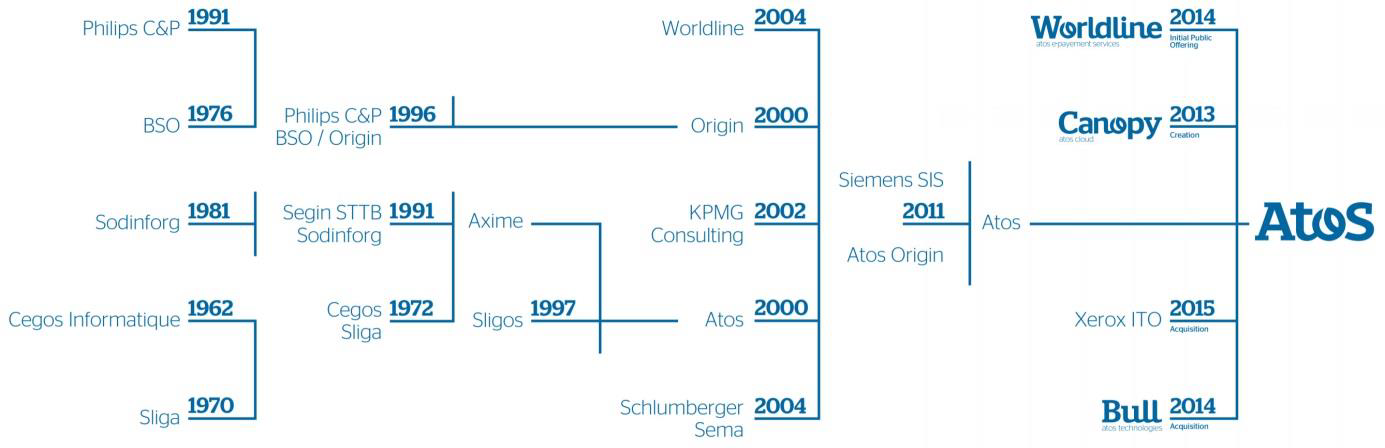
\includegraphics[width=0.99\textwidth]{img/Atos_acquisition_filiale.png}
	    \caption{Acquisitions et filiales d'Atos\cite{TweetAtosAcquisition}}
	    \label{fig:atos_acquisition}
	\end{figure}
	
	Atos étend ses activités par le biais d'acquisitions succéssives, parmis lesquelles on retrouve :\vspace{-1.5em}
	\begin{itemize}[itemsep=-0.5em]
	    \item L'infogérence et le conseil
	    \item Le cloud
	    \item Les services de e-paiement avec sa filiale Wordline
	    \item La cybersécurité
	    \item La défense et les sytèmes critiques
	\end{itemize}
	
	Atos est également le partenaire de grands groupes tel que Microsoft, Cisco et Oracle afin de pouvoir fournir au client des solutions innovantes.
	
	\newpage
	
	\section{Le groupe ÉS}
	Le groupe \acrshort{es} (\acrlong{es}), énergéticien régional multi-énergies en Alsace depuis plus de 100 ans et filiale d'EDF, fait partie des grands acteurs du secteur énergétique français. Le groupe, organisé autour de trois grandes activités, est composé :
	\begin{itemize}
	    \item d’un opérateur et gestionnaire de réseaux : Strasbourg Électricité Réseaux
	    \item d'une filiale commerciale : ÉS Énergies Strasbourg
	    \item de deux filiales spécialisées dans les services énergétiques et les énergies renouvelables : ÉS Services Énergétiques et ÉS Géothermie
	\end{itemize}
	
	\begin{figure}[ht]
	    \centering
	    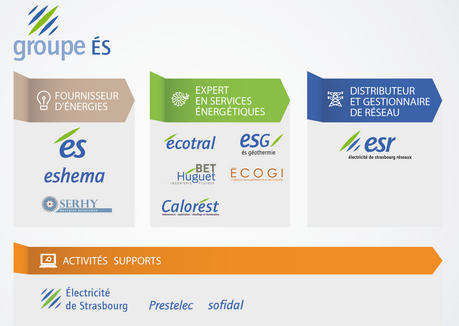
\includegraphics[width=0.9\textwidth]{img/orga_ES.png}
	    \caption{Organisation du groupe \acrshort{es}\cite{OrganisationES}}
	    \label{fig:orga_es}
	\end{figure}
	
	\newpage
	
	\section{Les activités d'Atos chez ÉS}
	Dans le cadre du contrat de \gls{tma} entre Atos (anciennement Bull) et \acrshort{es}, plusieurs équipes d'Atos sont présentent au centre opérationnel de Mundolsheim du groupe \acrshort{es}.
    Elles sont organisés en deux lots:
    \begin{itemize}
        \item Le lot 1, dont je fais partie, est chargé de la maintenance applicative et évolutive JAVA,  ainsi que des projets complémentaires.
        \item Le lot 2 est l’équipe décisionnelle.
    \end{itemize} 
    
    \subsection{Composition de l'équipe TMA JAVA}
    Le directeur de projet des équipes Atos est Gregory Bock.
    
    L'équipe \gls{tma} JAVA comprend 8 personnes:\vspace{-1em}
    \begin{itemize}[itemsep=-0.5em]
        \item MIGNON Sabrina, référant projet
        \item RICHARD Alexandre, référant TMA
        \item QUERE Alexandre
        \item TERREAUX Mathias
        \item MONTESANTOS Alexis
        \item GRILL Stéphane
        \item MARLIER David
        \item TURIN Gary
        \item BOUTET William
    \end{itemize}
    On distingue deux activités au sein de cette équipe :\vspace{-1em}
    \begin{description}
        \item[La \gls{tma} :] Consiste en la réalisation de correctifs en cas d'anomalies déclarées, et/ou d'évolutions mineures suite à une demande ou à l'évolution d'un logiciel.
        \item[Les projets :] Consiste en la création de nouvelles applications suivant le besoin du client.
    \end{description}
    
    Les utilisateurs déclarent les incidents via l'application PICTO. Ces demandes sont ensuite transférées au responsable de domaine fonctionnel qui valide l’incident et missionne la \gls{tma} pour le résoudre, suivant leurs ordre de priorité.
    
    \chapter{Environnements de travail}
    
    \section{Intégration à l'équipe}
    Durant la première semaine, j'ai suivi une formation concernant l'architecture \acrshort{rest} ainsi que sur l'environnement de développement JAVA utilisé par l'équipe. Nous utilisons entre autre les framework \gls{gwt} et \gls{gxt}.
    
    Ma charge de travail est répartie majoritairement sur du temps de projet.
    
    \section{Technologies utilisés}
    
    \subsection{Outils}
    L'équipe \gls{tma} JAVA a à sa disposition plusieurs \gls{vm}. Chaque développeur dispose donc du même environnement de travail. Suivant la version de \gls{gxt} utilisée, nous développons sur \gls{sts} pour \gls{gxt} 2 et sous \gls{eclipse} Mars pour \gls{gxt} 3.
    
    Nous avons également à notre disposition le logiciel PowerAMC, permettant de créer et modifier un modèle de base de données et de répercuter ces modificiations sur le \gls{sgbd}, ainsi que le logiciel SQL Developer nous permettant d'éxécuter des requêtes SQL sur la base de données. 
    
    Le navigateur cible des applications développées par l'équipe est Internet Explorer.
    
    \newpage
    
    Pour chaque projet nous utilisons un archetype \gls{maven} prédéfinis (application web ou \gls{webservice}), chaque application est séparées en plusieurs couches :\vspace{-1em}
    \begin{itemize}[itemsep=0em]
        \item Couche DAO : Gère l'accès aux bases de données et les requêtes.
        \item Couche Service : Effectue les traitements métiers, fait appel aux \glspl{webservice}
        \item Couche Server (application seulement) : Couche d'abstraction afin de faire appels au méthodes de la couche service.
        \item Couche RPC (application seulement) : Contient les interfaces synchrones et asynchrones des services de \gls{gwt}, les \gls{dto} et les classes utilitaires. Cette couche permet de faire le lien entre le client et le serveur.
        \item Couche RS (\gls{webservice} seulement) : Point d'entrée des méthodes de la couche service. Fait appels aux méthodes de la couche service.
        \item Couche Webapp (application seulement): Gère l'interface graphique, l'authentification et contient les ressources statiques de l'application (images, feuilles CSS, ...)
        \item Couche Interface (\gls{webservice} seulement) : Contient l'interface des services exposés par le \gls{webservice}.
    \end{itemize}\vspace{-0.5em}
    
    Nous utilisons également \gls{maven} pour gérer les dépendences des projets.\vspace{-0.5em}
    
    \subsection{Intégration continue et qualité de code}
    
    Afin d'améliorer la productivité et l'éfficacité des développeurs, plusieurs outils sont mis à notre disposition :
    \begin{itemize}[itemsep=0em]
        \item \gls{svn} : notre logiciel de gestion de versions
        \item Jenkins : logiciel open source d'intégration continue. Il permet de déployer rapidement et simplement les différents projets, mais peut également lancer des tâches définies, notamment afin de lancer un scan SonarQube via la même interface que pour les déploiements.
        \item SonarQube: SonarQube est un logiciel libre permettant de mesurer la qualité du code source à l'aide de nombreuses règles définies. SonarQube lance régulièrement une analyse des différents projets afin d'afficher la qualité générale du code, proposant ensuite des solutions aux bugs potentiels (pointeur null par exemple) et mauvaises pratiques et des améliorations concernant la lisibilité du code, notamment via les règles de codage (indentation, conventions de nommage, etc...).
    \end{itemize}
    
    Ces logiciels nous permettent d'une part de travailler en groupe, d'autre part d'améliorer la qualité des projets en général, les rendant plus facilement maintenable, mais aussi et surtout ils nous permettent d'être réactifs, c'est-à-dire de pouvoir traiter et corriger plus de problèmes avant que les utilisateurs n'y soient confrontés.
    
    \subsection{GWT / GXT}
    Pour développer l'\acrfull{ihm} des applications web, nous utilisons les frameworks \gls{gwt} et \gls{gxt}. Ceci nous permet d'utiliser une langage objet de haut niveau (en l'occurence JAVA) ainsi que les outils disponibles pour ce language (débuggers, bibliothèques). En resumé, ces deux framework nous permettent de développer nos applications de la même manière qu'une application JAVA Swing\footnote{Bibliothèque graphique JAVA}, à ceci près que l'on utilise les widgets de GWT et de GXT pour former l'interface. Ensuite le compilateur de GWT transforme le code JAVA en code Javascript tout en gérant la compression des ressources (images, texte, etc...), la gestion du cache et des appels \gls{ajax}.
    
    \subsection{Base de données et persistance des données}
    Nous utilisons le \gls{sgbd} Oracle pour stocker les données persistantes des applications. La gestion de la sauvegarde, suppression, mise à jour, et même le filtrage des différents objets sont effectués à l'aide du framework \gls{hibernate}. Pour ce faire chaque objet persistant se voit lié à une entité et un \gls{dao} dont tous les champs sont mappés\footnote{Signifie ici faire correspondre.} à une colonne d'une table à l'aide d'\gls{hibernate}. Cette table servira donc à stocker chaque objet d'une même classe JAVA.
    
    \chapter{Projets}
    
    \section{Histo-versions}
    L'application histo-versions a été le premier projet qui m'a été confié. Le but de cette application est d'afficher l'historique des déploiements des différentes applications pour chaque environnement. Afin d'éviter tout malentendu, sauf mention contraire, nous parlerons de création et de suppression d'application au sein d'histo-versions en parlant de l'ajout ou la suppression de lignes dans la table listant les applications, utilisée par histo-versions.
    
    \begin{figure}[ht]
        \centering
        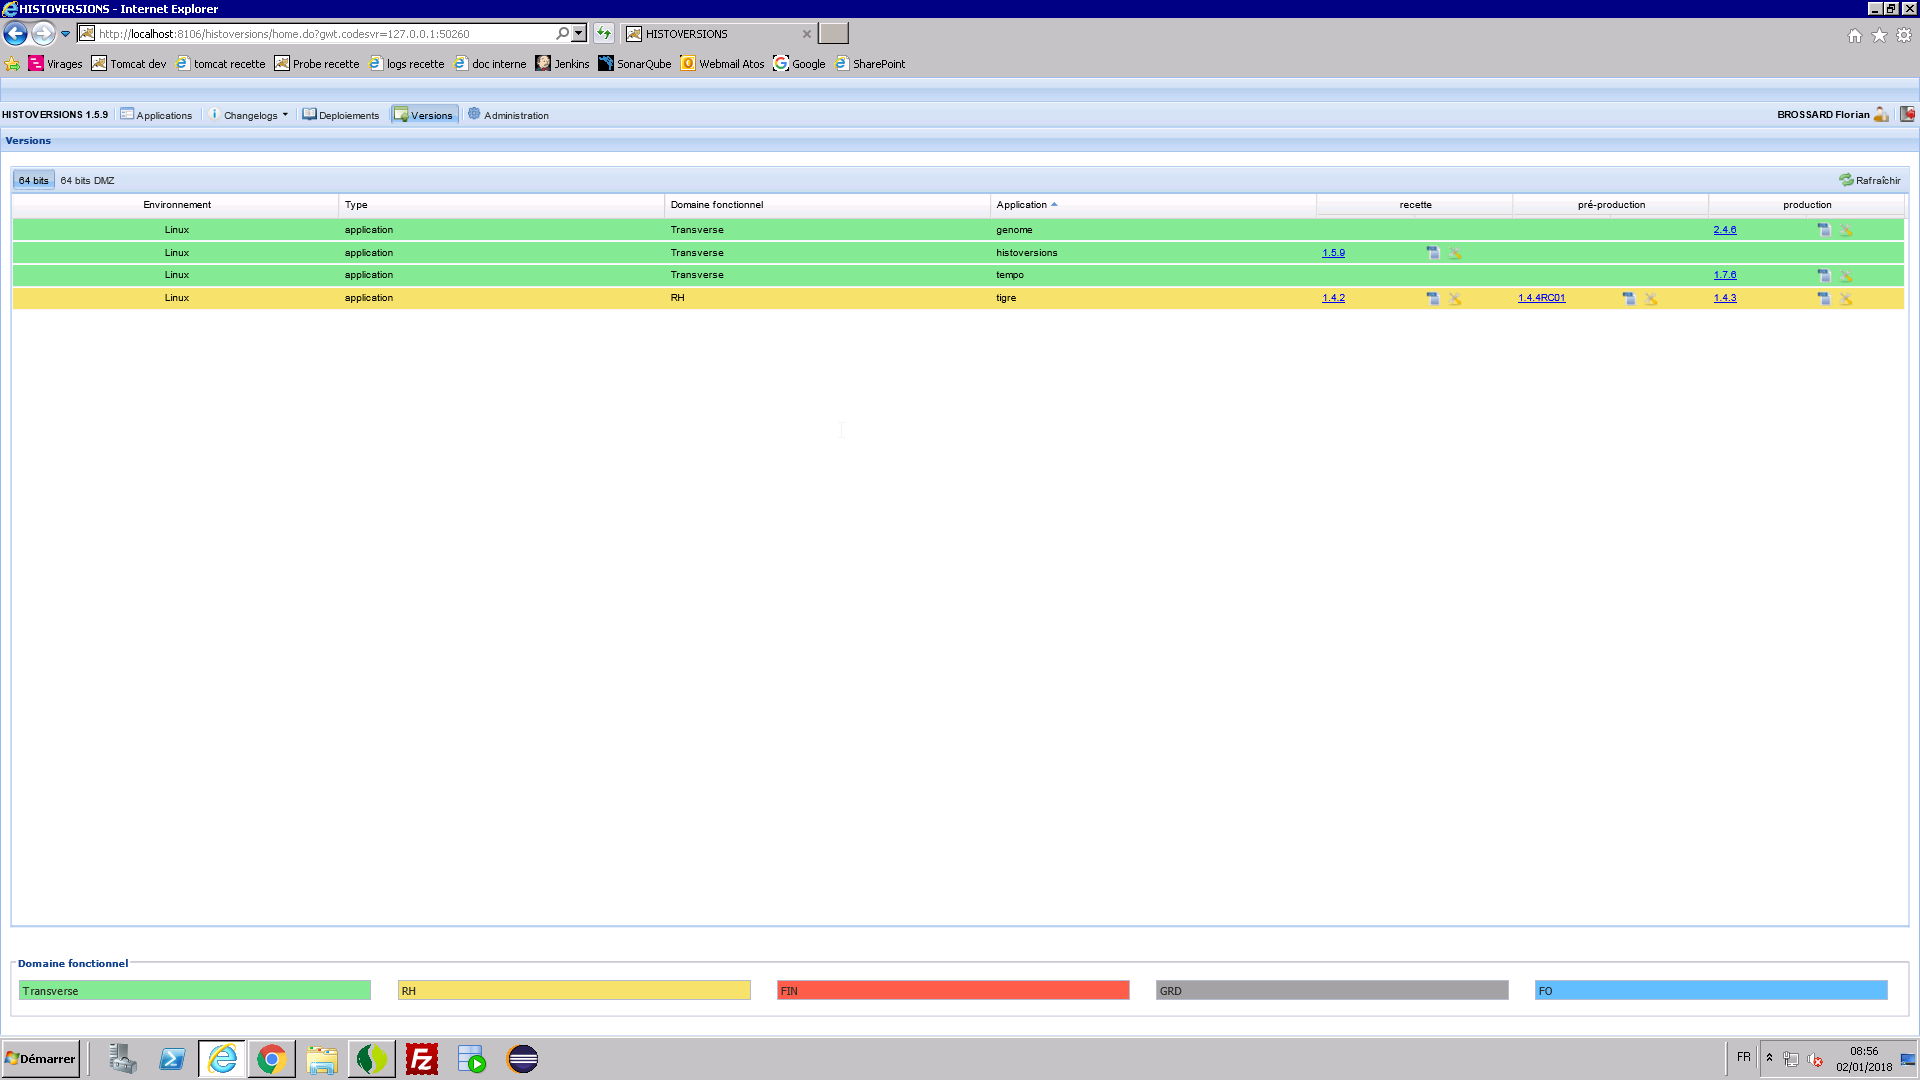
\includegraphics[height=8.2cm]{img/HV_Panel_versions.png}
        \caption{Panneau "applications" d'histo-versions}
        \label{fig:histoversions_versions}
    \end{figure}
    
    \subsection{Les environnements}
    Voici le cheminement du déploiement d'une nouvelle version d'une application:\vspace{-1em}
    \begin{enumerate}
        \item Lorsque le développement d'une évolution ou d'un correctif est terminé, une nouvelle version est déployée sur l'environnement dit de \textbf{recette}. Notre équipe a pleinement accès à cet environnement afin de déployer une nouvelle version.
        \item Suite à la confirmation du chef de projet et du responsable de domaine fonctionnel l'application peut, suite à des tests, être déployée sur l'environnement dit de \textbf{production}. C'est l'environnement qu'utilisent les utilisateurs.
        \item Éventuellement, une application peut être placée dans une environnement dit de \textbf{pré-production} si cela est nécessaire.
    \end{enumerate}
    
    \subsection{Fonctionnalités attendues}
    Voici une liste des fonctionnalités de l'application:\vspace{-1em}
    \begin{itemize}
        \item Afficher la liste des applications avec le numéro de la version déployée pour chaque environnement (\textbf{recette, pré-production, production} et leur équivalent \textbf{\gls{dmz}})
        \item Afficher la liste des changelogs\footnote{Un changelog, ou journal des modifications, est une liste des modifications\cite{wiki:changelog}.} pour chaque application
        \item Afficher la liste de tous les déploiements de chaque application dans chaque environnement
        \item Pouvoir effectuer plusieurs opérations dont la sélection des applications à afficher, l'ajout/suppression de ces applications et des changelogs dans histoversions et le filtrage des applications (par nom, version, environnements, etc...)
    \end{itemize}
    
    \newpage
    
    \subsection{Travail effectué}
    
    Afin de me familiariser avec le projet ainsi qu'avec les méthodes de travail, j'ai débuté une amélioration de la qualité du code évaluée par SonarQube. Cela m'a permis d'apprendre à me servir des outils mis à ma disposition (svn, Jenkins, SonarQube, ...) et à utiliser les différents frameworks.
    
    Plusieurs réécritures de morceaux de codes, de classes, ainsi que l'ajout de classes utilitaires ont dans un premier temps permis de rendre le code plus court, en évitant les répétitions, et plus clair, en renommant certaines fonctions et variables ambiguës. Ces changements ont également permis de résoudre certains bugs.
    
    Mes premières tâches, en dehors de l'amélioration de la qualité de code, ont été de régler quelques problèmes concernant l'interface.
    Voici un exemple concret avec une capture d'écran montrant l'interface d'histo-versions sur l'écran de création et suppression des applications :
    \begin{figure}[ht]
        \centering
        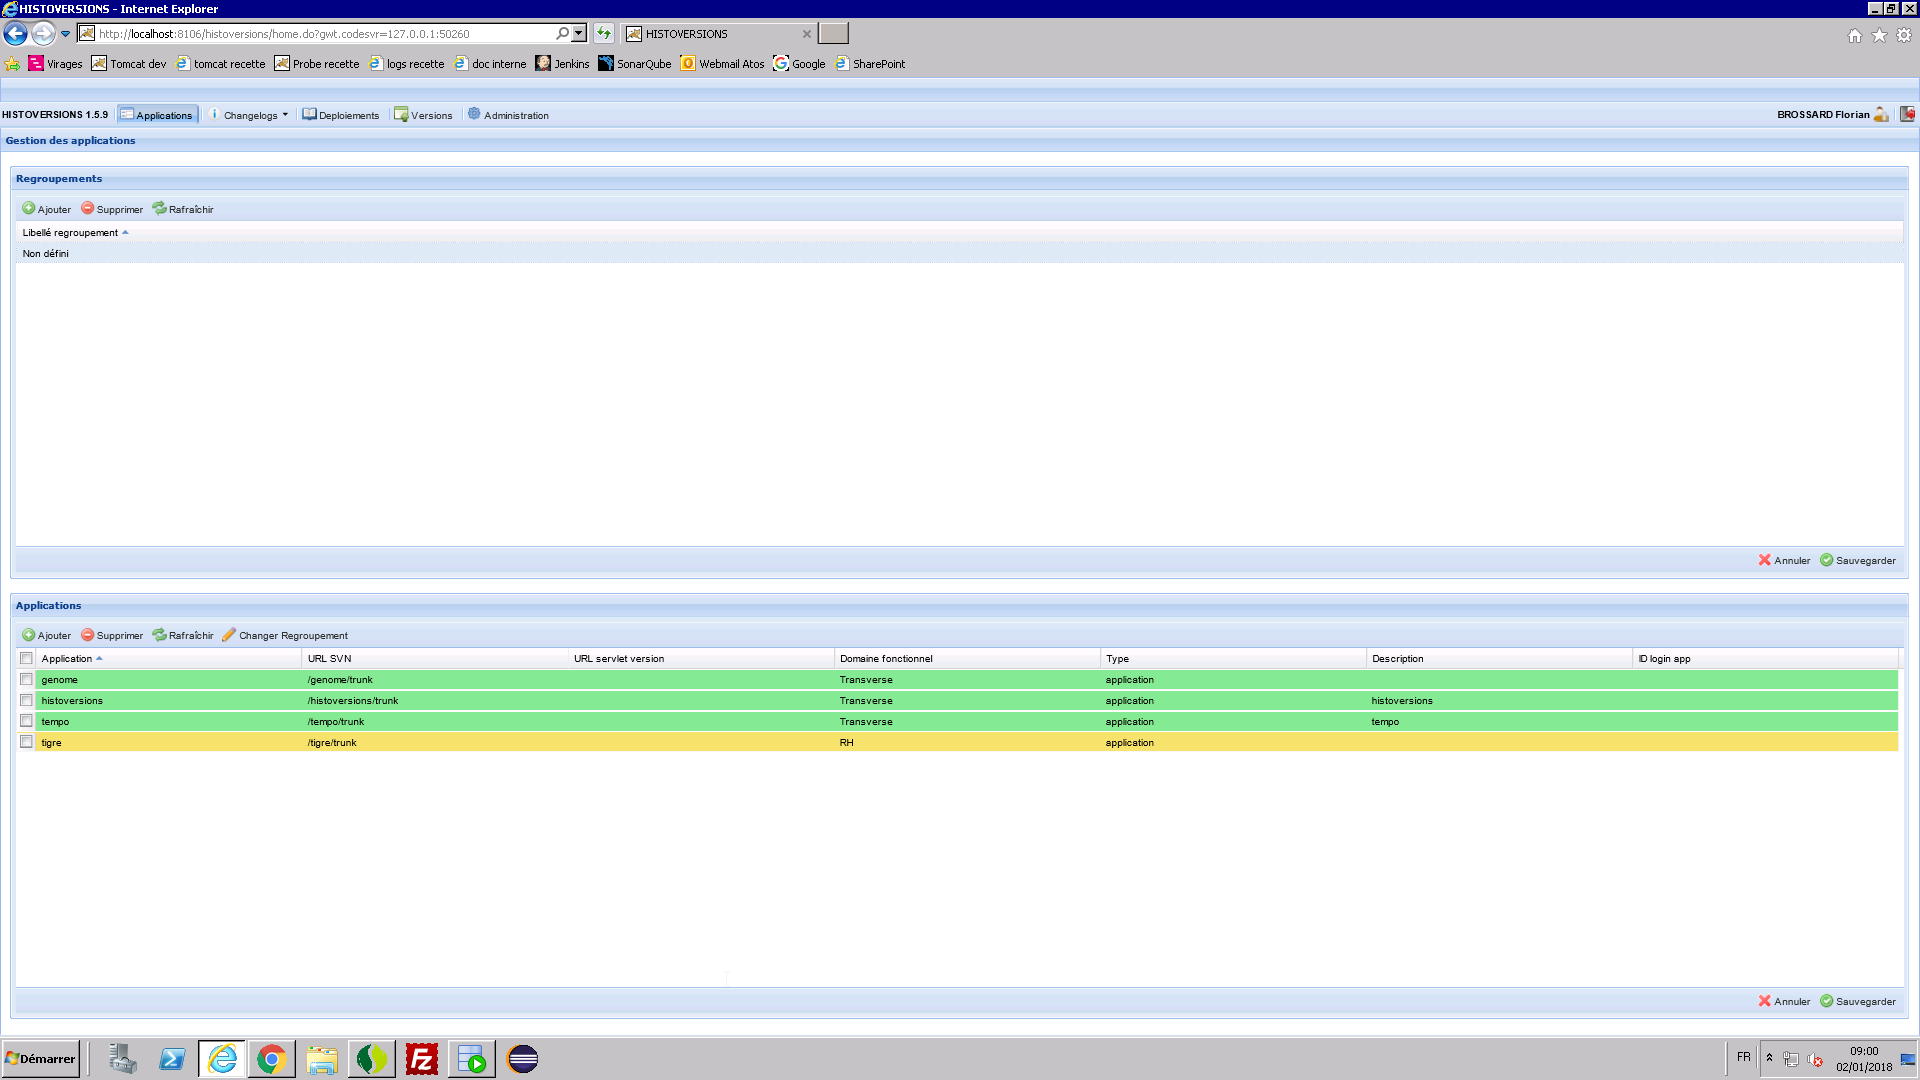
\includegraphics[width=0.99\textwidth]{img/HV_Panel_applications.png}
        \caption{Panel "Applications"}
        \label{fig:histoversions_applications}
    \end{figure}
    
    Chaque ligne présente dans ces deux grilles est une ligne présente dans une table (ou une vue) de la base de donnée. Afin de garder une trace des suppressions dans la base de données, chaque table possède une colonne ETAT\_OBJET prenant la valeur 0 ou 1, représentant respectivement un objet supprimé logiquement ou non.
    
    Cet écran, ainsi que d'autres, présentant entre autres les versions, les changelogs et les déploiements des application, affichaient toutes les lignes quel que soit leur état. Le problème était dû à une vérification manquante d'une des colonnes ETAT\_OBJET, et à l'utilisation d'une requête SQL native plutôt qu'à l'utilisation d'une vue existante.
    
    D'autres légers changements ont été effectués concernant l'interface afin de la rendre plus lisible et plus claire, et quelques autre bugs mineurs (c'est à dire non bloquants) ont été corrigé, tel que l'affichage d'une erreur lorsque l'utilisateur souhaite supprimer une ligne venant d'être ajoutée à la grille des applications, sans avoir validé l'ajout au préalable.
    
    Une autre tâche à été de rendre périodique l'ajout automatique des déploiements dans la base de donnée. Cet ajout est réalisé à l'aide d'un batch\footnote{En informatique, un traitement par lots (batch processing en anglais) est un enchaînement automatique d'une suite de commandes (processus) sur un ordinateur sans intervention d'un opérateur\cite{wiki:batch}} JAVA. Pour ce faire j'ai dû modifier ce batch afin de pouvoir l'utiliser en tant que tâche, au lieu d'être utilisé en tant que webservice, accessible depuis un lien web. Ceci a également permis de s'affranchir de l'ouverture d'une nouvelle fenêtre contenant uniquement le résultat de l'éxécution, c'est à dire le nombre d'erreurs rencontrées, lors de son éxécution manuelle. Le résultat est maintenant affiché dans une boîte de dialogue directement intégrée à l'application.
    
    \newpage
    
    \section{pApps}
    Dans le cadre de mon apprentissage et de ma formation, le projet pApps m'a été confié.
    
    Le projet pApps (pour portail applications) est né d'un besoin de proposer aux utilisateurs un portail d'accès centralisé aux applications. Ce projet remplacera donc l'actuel accès aux applications par leurs adresses.
    
    \subsection{Fonctionnalités demandées}
    Voici la liste des fonctionnalités demandées:\vspace{-1em}
    \begin{itemize}
        \item Afficher une liste des applications
        \item N'afficher que les applications auxquelles l'utilisateur a accès
        \item Afficher, si possible, une icone représentant l'application
        \item Afficher l'environnement des applications
        \item Pouvoir signaler un problème sur une application via le logiciel PICTO en passant par ce portail
    \end{itemize}
    
    Afin de répondre à ces attentes, nous pouvons utiliser un webservice deja existant permettant de lister les applications auxquelles l'utilisateur a accès. Les icônes des applications peuvent être recherchées sur le serveur, en supposant que l'on respecte un certain formattage du nom des fichiers. Dans le cas où une image n'est pas trouvée, on peut la remplacer par une image par défaut, le logo du groupe \acrshort{es} par exemple.
    
    \newpage
    
    \subsection{Interface}
    Concernant l'affichage des environnements des applications, nous avons imaginé deux solutions:\vspace{-1em}
    \begin{itemize}
        \item Plusieurs onglets regroupant chacun les applications d'un seul environnement, avec le nom de l'environnement en guise de label pour l'onglet
        \item Si l'on considère que chaque application est représentée par une tuile, on mettre une couleur de fond et un motif à cette tuile pour indiquer l'environnement.
    \end{itemize}
    On peut aussi combiner ces deux solutions en mettant par exemple une légende à un endroit visible de la fenêtre, indiquant pour chaque couleur le nom de l'environnement. Chaque élément de cette légende étant cliquable, on peut appliquer un filtrage sur les environnements.
    
    C'est d'ailleurs cette solution que j'ai proposée en premier lieu:
    
    \begin{figure}[ht]
        \centering
        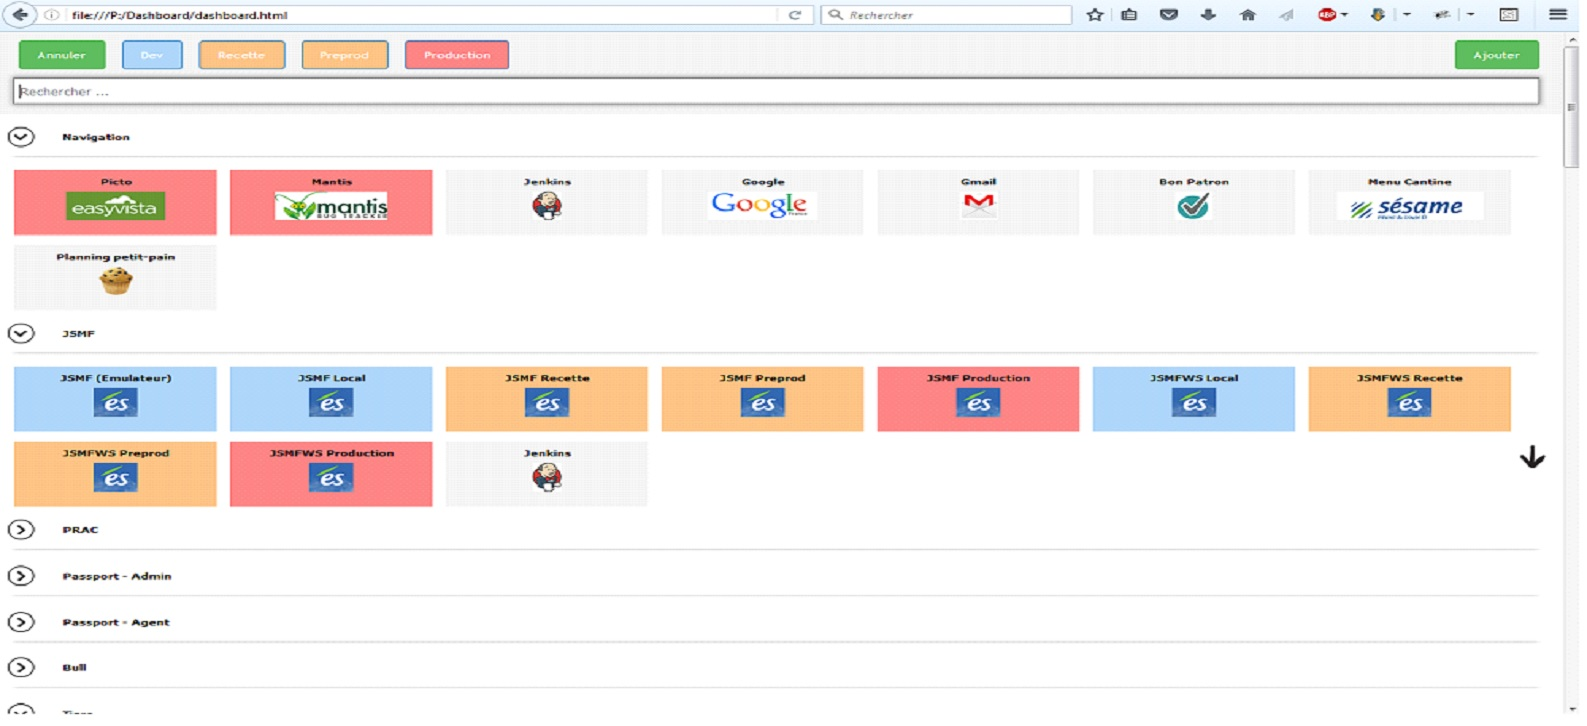
\includegraphics[width=0.99\textwidth]{img/interface_proposition_sfd.jpg}
        \caption{Interface proposée pour pApps}
        \label{fig:papps_interface}
    \end{figure}{}
    
    \newpage
    
    \subsection{Travaux en cours}
    À l'heure actuelle, l'interface n'est pas encore terminée. Une grande partie du travail est de trouver et modifier les différents styles CSS afin de rendre le tout plus esthétique.
    
    Concernant le développement du projet, au lieu d'adopter le modèle du cycle en V\footnote{Le modèle du cycle en V (en comparaison avec les méthodes dites agiles) est un modèle conceptuel de gestion de projet imaginé\cite{wiki:cycleV}.} habituel, nous avons décidé d'utiliser un modèle plus orienté méthode agile\footnote{Les méthodes agiles se veulent plus pragmatiques que les méthodes traditionnelles, impliquent au maximum le demandeur (client). Elles reposent sur un cycle de développement itératif, incrémental et adaptatif\cite{wiki:agile}.}. Ainsi, je peux organiser un rendez-vous rapidement avec le responsable de projet du groupe \acrshort{es}, afin de discuter et valider chaque partie de l'application une par une.

    \section{Futur projet}
    Pour le moment, en plus du projet pApps, plusieurs transferts de compétences sont prévus. Cela consistera entre autres à comprendre la partie métier visée par ces applications ainsi que leur conception. Je serai par la suite amené à gèrer les différents retours d'anomalies et évolutions demandées liés à ces applications.
    
    Mis à part cela, et étant donné la nature des activité d'Atos pour le groupe \acrshort{es}, il est difficile de prévoir la création de projet sur le long terme.
    
    \chapter{Bilan}
    Ce début d'expérience m'a permis de découvrir une nouvelle manière de concevoir une application. J'ai également appris à utiliser l'intégration continue, ce qui est un véritable avantage par rapport à mes précédents projets. Je m'aperçois que tout cela facilite énormément le développement d'un projet en évitant les problèmes de dernières minute et en donnant une manière de respecter certaines règles quant à l'écriture du code.
    
    Étant au sein d'une équipe compétente et agréable, je trouve toujours réponse à mes questions et j'ai toujours plaisir à travailler.
    
    Tout cela à été très formateur et m'a permis d'en apprendre beaucoup concernant l'informatique et le développement logiciel.
    
	\fin
	
	%Résumé
    \printAbstract{
        Dans le cadre de mon Master informatique \acrlong{ilc}, j'ai effectué mon apprentissage au sein du groupe Atos.
        \p
        Ce mémoire présentent les groupe Atos et \acrshort{es}, ainsi que les premiers mois de mon travail pour \acrshort{es} dans l'équipe Atos.
    }
    {Atos, \acrshort{es}, Application Web, GXT, GWT, REST}
    {
        Through my Master degree in computer science, I worked within the Atos group under an apprenticeship contract.
        \p
        This report presents the Atos and \acrshort{es} groups, as well as the first months of my work for the \acrshort{es} group within the Atos team.
    }
    {Atos, \acrshort{es}, Webapp, GXT, GWT, REST}
    
\end{document}
